% 1.1.3
\subsubsection{Phân loại kỹ thuật mã hóa: đối xứng và bất đối xứng}
\indent Trong lĩnh vực bảo mật thông tin, kỹ thuật mã hóa được chia thành hai loại chính: mã hóa đối xứng và mã hóa bất đối xứng. Hai mô hình này khác nhau chủ yếu ở cách sử dụng khóa trong quá trình mã hóa và giải mã, như thể hiện trong Hình ~\ref{fig:cdm2} dưới đây.

\begin{figure}[H]
  \centering
  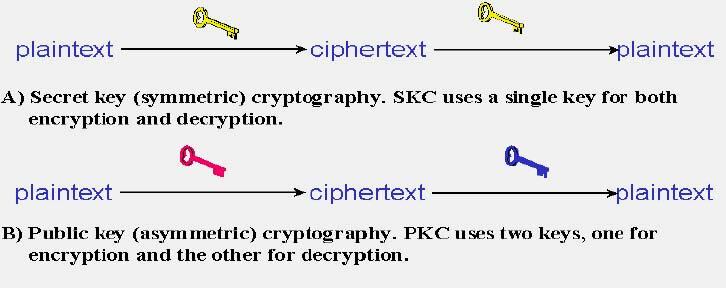
\includegraphics[width=.85\textwidth]{figures/pic2.png}
  \caption{Minh họa hai mô hình mã hóa trong bảo mật thông tin.}
  \label{fig:cdm2}
\end{figure}

\indent Phần (A) biểu diễn mã hóa đối xứng (Symmetric Key Cryptography) – sử dụng cùng một khóa duy nhất cho cả mã hóa và giải mã. Phương pháp này có ưu điểm là tốc độ nhanh và dễ triển khai, nhưng vấn đề an toàn nảy sinh khi phân phối khóa cho các bên tham gia, ở phạm vi đề tài này chúng tôi sẽ dùng khóa bất đối xứng RSA để thực hiện trao đổi khóa AES an toàn.

\indent Phần (B) mô tả mã hóa bất đối xứng (Asymmetric Key Cryptography) – sử dụng hai khóa riêng biệt: khóa công khai (public key) và khóa bí mật (private key) tùy thuộc vào mục đích sử dụng mà có thể dùng khóa public private để mã hóa hay giải mã thông tin. Cách tiếp cận này giúp giải quyết khó khăn trong việc chia sẻ khóa, đồng thời tăng cường tính xác thực và an toàn cho hệ thống, dù tốc độ xử lý chậm hơn mã hóa đối xứng.